\documentclass[informe.tex]{subfiles}
\begin{document}

\textbf{Definición}\newline

La función de transferencia de un filtro FIR tiene la forma:

$$
	H(z) = \sum_{n=0}^{N}{h(n)z^{-n}}
$$

$h(n)$ es una secuencia que representa la respuesta al impulso en tiempo discreto, de longitud finita y causal.\\

Hay varias formas de diseñar un filtro FIR, una forma es por truncamiento de la respuesta al impulso, y la otra forma puede ser por muestreo de frecuencia.\\

Aquí se desarrolla solo el primer método. En este método se especifica la respuesta en frecuencia, $H(j\omega)$, y luego se plantea la serie de Fourier de ésta (en $j\omega$), la secuencia resultante representa la respuesta al impulso en tiempo discreto, $h_d(n)$. Como esta secuencia tiene duración infinita y es no causal, se multiplica por una ventana tal que trunque la secuencia fuera de los límites de dicha ventana, y finalmente se desplaza de tal modo que quede causal.\newline

En base a lo dicho al párrafo anterior, $h(n)$ va ser una secuencia de tiempo de discreto causal y de longitud $N$ finita, y esto hace que se  se den cuatro tipos o casos de simetrías.\\\\
- Tipo I: Simetría respecto a $\pi$ con una cantidad $N$ impar de muestras.\\
- Tipo II: Simetría respecto a $\pi$ con una cantidad $N$ par de muestras.\\
- Tipo III: Anti simetría respecto a $\pi$ con una cantidad $N$ impar de muestras.\\
- Tipo IV: Anti Simetría respecto a $\pi$ con una cantidad $N$ par de muestras.\\

Para el tipo II y IV solo es aplicable a filtros pasa bajos y pasa medios, y los otros tipos no tienen restricciones. Para que el filtro fuese de fase lineal $h(n)$ debe cumplir la condición:
  $$ h(n) = h(N-1-n)$$
y esto asegura también que sea causal.\\

Otra característica de la aproximación por truncamiento de la respuesta del impulso ideal es que se da el fenómeno de convergencia no uniforme de Gibbs en la discontinuidades. En este sentido se utilizan diferentes ventanas para atenuar dichos sobre-impulsos.\\\\

\underline{Desarrollo}\\

Para comenzar con la aproximación por truncamiento de la respuesta del impulso se especifica el filtro ideal en el dominio de la frecuencia, 
	$$
		H(j \omega T= j\Omega) = \begin{cases}
									1  & |\omega T| < \omega_c T=\Omega_c \\
									0  & \mbox{para otro valor}						
								 \end{cases}
	$$
donde $\Omega=\omega T$	 es la frecuencia normalizada de $\omega$ con respecto a la frecuencia de muestreo $1/T$, entonces $\Omega$ va variar entre $-\pi$ y $\pi$; $\Omega_c$ es la frecuencia de corte normalizada, y  $\omega_c$ es la frecuencia de corte no normalizada.\\

Se supone que $H(j\Omega)$ es periódica de período $2\pi$, quedando el desarrollo en serie de Fourier de la respuesta en frecuencia $H(j\Omega)$, representada en la Fig. \ref{fig:fir:representacion_Hs}, tal como
	$$
		H(j\omega T= j\Omega) = \sum_{-\infty}^{n=\infty}{b_n e^{-j \cdot 1 \cdot n}}
	$$
donde la frecuencia fundamental es $1$, entonces $\omega_0 = \frac{2\pi}{2\pi}=1$.
		\begin{figure}[h!]
		\centering
		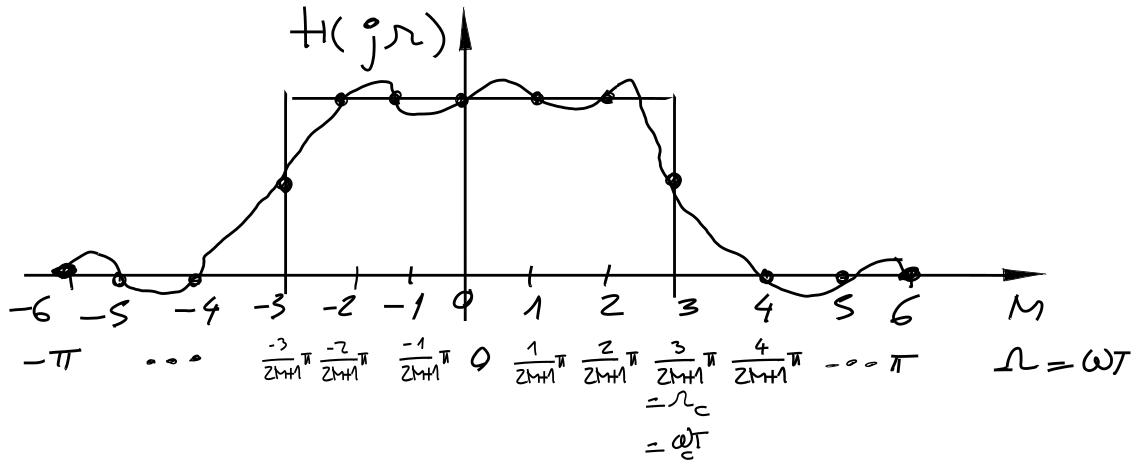
\includegraphics[scale=0.4]{fir_resp_freq_serie.jpg}
		\caption{Representación gráfica de $H(j\omega)$ y de su desarrollo serie de Fourier en $j\omega$}
		\label{fig:fir:representacion_Hs}
		\end{figure}
En este caso, $b_n$ se asocia directamente con la secuencia en tiempo discreto $h_d(n)$, Fig. \ref{fig:fir:representacion_Hs}, y que corresponde a los coeficientes de $H(j\omega)$.\\
	$$
		h_d(n) = b_k = \frac{1}{2\pi} \int_{-\Omega_c}^{\Omega_c}
		                                  {1 \cdot e^{-j 1 \cdot n \Omega}}
		           = \frac{ sin( \Omega_c n )}{ \pi n}
	$$
		\begin{figure}[h!]
		\centering
		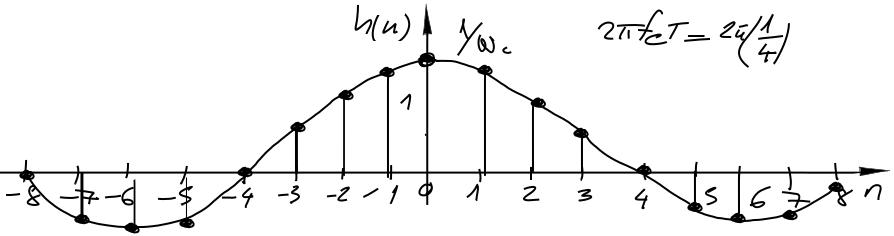
\includegraphics[scale=0.4]{fir_resp_impulso.jpg}
		\caption{Representación gráfica de la respuesta al impulso $h_d(n)$.}
		\label{fig:fir:representacion_hdn}
		\end{figure}
Esta secuencia, $h(n)$ tiene una cantidad infinita de términos y además no es causal. Una forma de resolver la causalidad es multiplicar esta secuencia por una ventana que trunque la secuencia a una cantidad de términos diferentes de cero y luego desplazar esta secuencia de tal forma que quede causal. En primera instancia la ventana $w(n)$ puede ser una ventana rectangular de longitud $N$, tal como se muestra trazada en rojo en la Fig. \ref{fig:fir:representacion_venta_rectangular}.
	\begin{equation}
		\label{eqn:fir:ventana}	
		h(n) = h_d(n) \cdot w(n)
	\end{equation}
    \begin{figure}[h!]
		\centering
		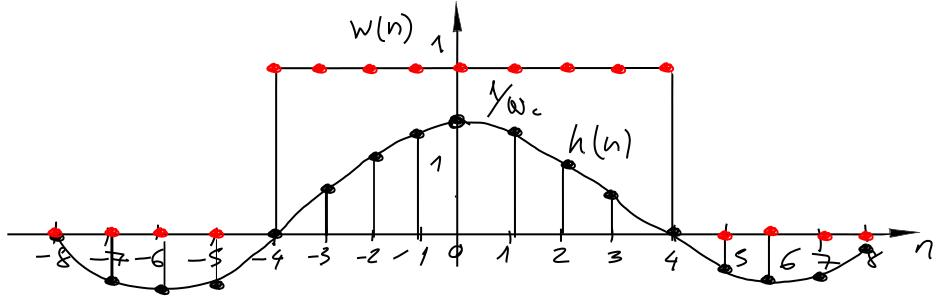
\includegraphics[scale=0.5]{fir_ventana.jpg}
		\caption{Representación gráfica de $h_d(n)$ y $w(n)$ (trazado en rojo)}
		\label{fig:fir:representacion_venta_rectangular}
	\end{figure}

Finalmente, a partir de la Ec. \ref{eqn:fir:ventana}, $h(n)$ será una secuencia de longitud N finita y casual, lo que para un $N$ par la expresión quedaría definida como:
	\begin{equation}
		\label{eqn:fir:sec_impar}	
		h\left(n\right)=
			\begin{cases}
				\frac{ 
			     sin \left( \Omega_c \pi \left( n - \frac{N-1}
			                                            {2} \right) \right)}
				  {\pi \left( n - \frac{N-1}{2} \right)}	
				  & \mbox{para }n != \frac{N-1}{2}
			\\
			\Omega_c & \mbox{para }n=\frac{N-1}{2}
			\end{cases} 
	\end{equation}

En la Fig. \ref{fig:fir:sec_impar} representa el caso de longitud impar dado en la Ec. \ref{eqn:fir:sec_impar}.\newline
\begin{figure}[h]
		\centering
		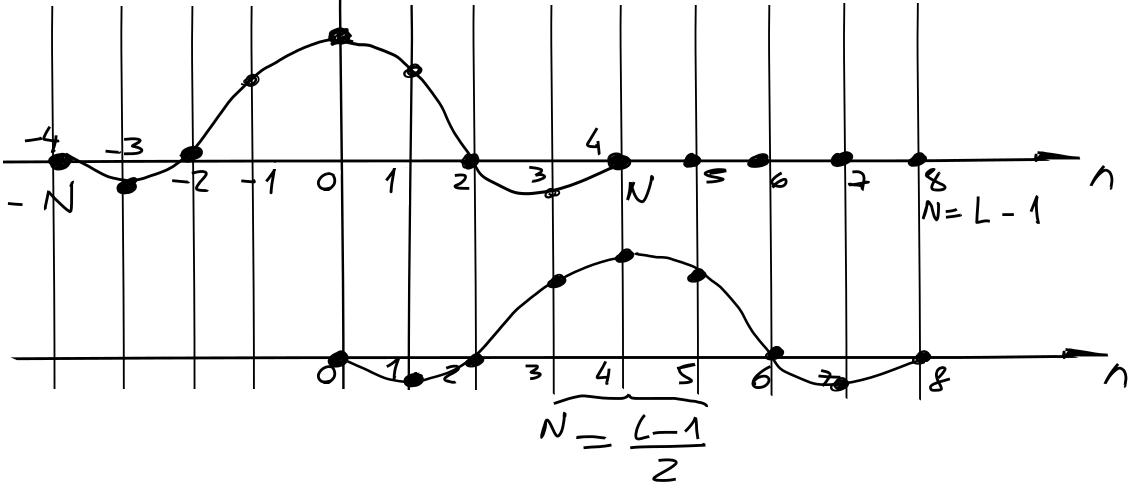
\includegraphics[scale=0.3]{fir_sec_impar.jpg}
		\caption{Representación de $h_d(n)$ y de $h(n)$ para $N$ impar.}
		\label{fig:fir:sec_impar}
\end{figure}

Y para una secuencia $h(n)$ de $N$ par se tiene:
	\begin{equation}
		\label{eqn:fir:sec_par}	
		h\left(n\right)=
				\frac{ 
			     sin \left( \Omega_c \pi \left( n - \frac{N-1}
			                                            {2} \right) \right)}
				  {\pi \left( n - \frac{N-1}{2} \right)}	
	\end{equation}

En la Fig. \ref{fig:fir:sec_par} representa el caso de longitud par dado en la Ec. \ref{eqn:fir:sec_par} .\newline

	\begin{figure}[h]
		\centering
		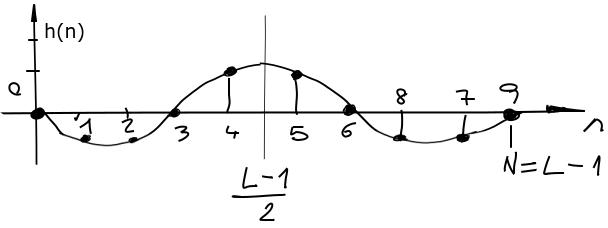
\includegraphics[scale=0.4]{fir_sec_par.jpg}
		\caption{Representación de $h_d(n)$ y de $h(n)$ para $N$ par.}
		\label{fig:fir:sec_par}
	\end{figure}

%%
\textbf{Ejemplo con Matlab 1:} Filtro pasa bajos FIR, Fig. \ref{fig:fir:freqz_ej1}.\newline    

\lstinputlisting[language=MATLAB, frame=single]{./src_matlab/fir1_ej1.m}
	
	\begin{figure}[h]
		\centering
		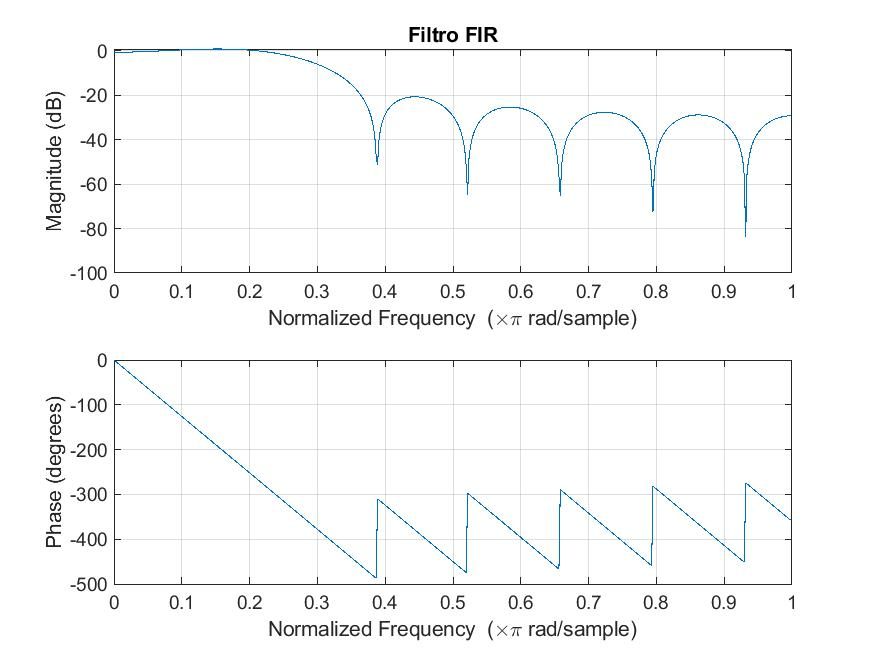
\includegraphics[scale=0.4]{fir1_ej1.jpg}
		\caption{Respuesta en frecuencia.}
		\label{fig:fir:freqz_ej1}
	\end{figure}	

%%
\textbf{Ejemplo con Matlab 2:} Filtro pasa altos FIR, Fig. \ref{fig:fir:freqz_ej2}.\newline    

En este ejemplo se construyó una función que permita determinar el filtro y posibilite elegir el tipo de filtro y el tipo de ventana a aplicar al mismo.

\lstinputlisting[language=MATLAB, frame=single]{./src_matlab/mi_fir1.m}

A continuación se muestra el uso de esta función con un ejemplo:

\lstinputlisting[language=MATLAB, frame=single]{./src_matlab/fir1_ej2.m}
	
	\begin{figure}[h]
		\centering
		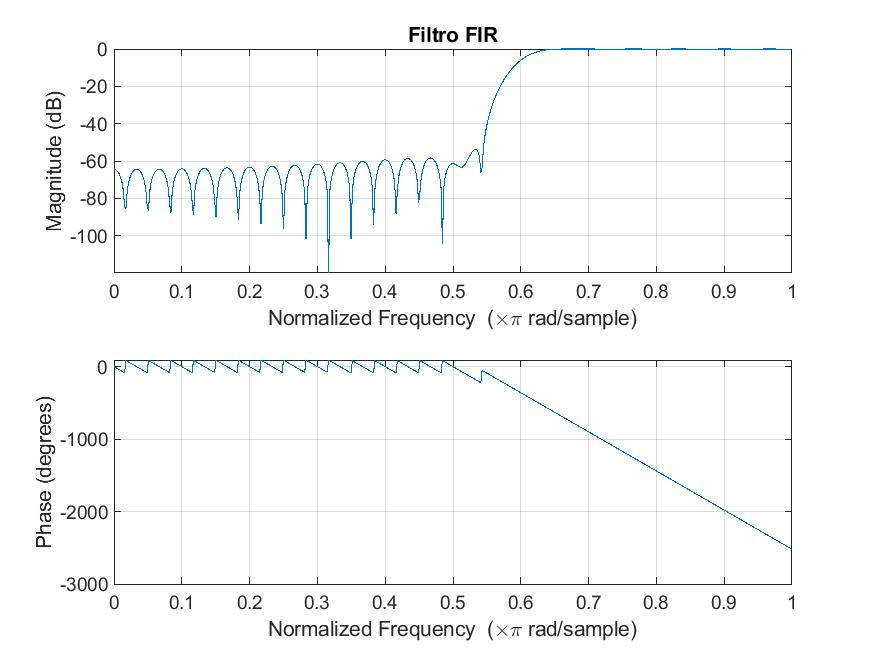
\includegraphics[scale=0.4]{fir1_ej2.jpg}
		\caption{Respuesta en frecuencia.}
		\label{fig:fir:freqz_ej2}
	\end{figure}
	
\end{document}	